\fancyfoot[C]{Sandri}
\section{Elektrische Antriebsmaschinen} \label{Motoren}
Elektrische Maschinen wandeln elektrische Energie in mechanische Energie um, indem sie das Prinzip der Lorenzkraft beziehungsweise Reluktanzkraft anwenden um einen Rotor zu rotieren. Der grunds�tzliche Aufbau eines elektrischen Motors besteht grunds�tzlich aus einem Stator, dem nicht-rotierendem Teil, und einem Rotor, dem sich rotierenden teil. Je nach Typ und Ausf�hrung des Motors sind auf beiden Komponenten Wicklungen beziehungweise Dauermagnete befestigt. Bei einigen Motoren sind auch noch andere Bauteile verbaut.

\subsubsection{Lorentzkraft}
	Die Lorentzkraft wirkt auf bewegliche Lasungstr�ger in einem Magnetfeld. Sie wirkt senkrecht zur Bewegungsrichtung der Ladung und senkrecht zu den Feldlinien des Magnetfelds. Wie sich die Lorentzkraft verh�lt, l�sst sich anhand folgendem Beispiel, einer Leiterschaukel erkl�ren:

	\begin{figure}[H]
			\centering
			\includegraphics[scale=0.8]{./3_Stand_der_Technik/Abbildungen/Leiterschaukel_1}
			\caption{�nderung der Stromrichtung Lorentzkraft\cite{schullv.de2024}}
	\end{figure}
	
	Die Richtung in welche die Leiterschaukel ausschl�gt, ist zum einen Abh�ngig von der Richtung des Stroms und zum anderen von der Orientierung des Magnetfelds.
	
	\begin{figure}[H]
			\centering
			\includegraphics[scale=0.8]{./3_Stand_der_Technik/Abbildungen/Leiterschaukel_2}
			\caption{�nderung des Magnetfelds Lorentzkraft\cite{schullv.de2024}}
	\end{figure}
	
	Die Richtung der Lorentzkraft kann auch durch einen einfachen Versuch, den linke Hand Versuch, ermittelt werden:
	
	\begin{figure}[H]
			\centering
			\includegraphics[scale=0.8]{./3_Stand_der_Technik/Abbildungen/Lorentzkraft_1}
			\caption{Die linke Hand Regel\cite{schullv.de2024}}
	\end{figure}

	Mathematisch kann die Richtung der Lorentzkraft mihilfe des Kreuzprodukts aus der Magnetfeldrichtung und der Bewegungsrichtung der Elektronen errechnet werden:
	
	\begin{equation}
		\vec{F_{L}} = q * (\vec{v_{e}} \times \vec{B})
	\end{equation}
	
	Der Betrag kann wiefolgt errechnet werden:
	
	\begin{equation}
		F_{L} = q*v*B*\sin{\alpha}
	\end{equation}
	
	Wobei der Winkel $\alpha$ den Winkel zwischen der Bewegungsrichtung der Elektronen und der Bewegungsrichtung des Magnetfelds entspricht. Auch kann man anhand dieser Formel erkennen, dass die Lorentzkraft null wird, wenn die Bewegungsrichtung der Elektronen und die des Magnetfelds parallel verl�uft.\cite{schullv.de2024}
	
	Die meisten elektrischen Maschinen funktionieren grunds�tzlich aufgrund der Lorentzraft, es gibt jedoch vereinzelt Maschinen, die nur aufgrund der Reluktanzkraft funktionieren.

\subsubsection{Reluktanzkraft}

	Die Reluktanzkraft (auch Maxwellsche Kraft genannt) entsteht durch �nderung des magnetischen Widerstands. Sie wirkt immer so, dass sich der magnetische Widerstand verringert und die Induktivit�t steigt. Diese Kraft kann durch Ver�nderung des Luftspalts im magnetischen Kreis erzeugt werden.\cite{biancahoegel.de/2021}
	
	\subsection{Asynchronmaschine}
	Die Asynchronmaschine ist die einfachste Form einer elektrischen Maschine. Sie wird angetrieben durch ein Drehfeld, welches durch eine mehrstr�ngige Wicklung im Stator erzeugt wird. Der gro�e Vorteil des Asynchronmaschine ist ihre einfache Bauform und Funktionsweise. Auch bedarf sie nur geringer Wartung. Der gro�e Nachteil hingegen ist jedoch seine startk an die Frequenz der Eingangsspannung gebundene Drehzahl. Im gebr�uchlichen 50-Hz-Betrieb sind nur Drehzahlen von 3000U/min, 1500U/min, 1000U/min, abh�ngig von der Anzahl der Polpaare.
	
	\begin{equation}
		n \thickapprox f / p
	\end{equation}
	
	n $\cdots$ Motordrehzahl \newline
	f $\cdots$ Frequenz vom Netz	\newline
	p $\cdots$ Anzahl der Polpaare \newline
	
	Es gibt haupts�chlich zwei Typen der Asynchronmaschine, den K�figl�ufer und den Schleifringl�ufer. Der K�figl�ufer verwendet also Rotor eines Stahlk�fig, der Schleifringl�ufer hat Schleifringe, �ber die Wicklungen im Rotor bestromt werden.
	
	\begin{figure}[H]
			\centering
			\includegraphics[scale=0.6]{./3_Stand_der_Technik/Abbildungen/Asynchronmaschine_2}
			\caption{Aufbau K�figl�ufer\cite{kfzaufgaben.de2024}}
	\end{figure}
	
	\begin{figure}[H]
			\centering
			\includegraphics[scale=2]{./3_Stand_der_Technik/Abbildungen/Asynchronmaschine_3}
			\caption{Aufbau Schleifringl�ufer\cite{wupperindustrie.de2024}}
	\end{figure}

	Betrieben wird die Asynchronmaschine indem sie an das 3-phasige 50Hz-Netz angeschlossen wird. Sie dreht sich dadurch fast synchron mit der Netzfrequenz. Asynchronmaschinen laufen ihrem Feld jedoch immer etwas hinterher, diese Eigenschaft nennt man Schlupf. Das Drehmoment- und Drehzahlverhalten kann sehr gut mittels eines Kreisdiagramms dargestellt werden.\cite{Fischer2017}
	
	\begin{figure}[H]
			\centering
			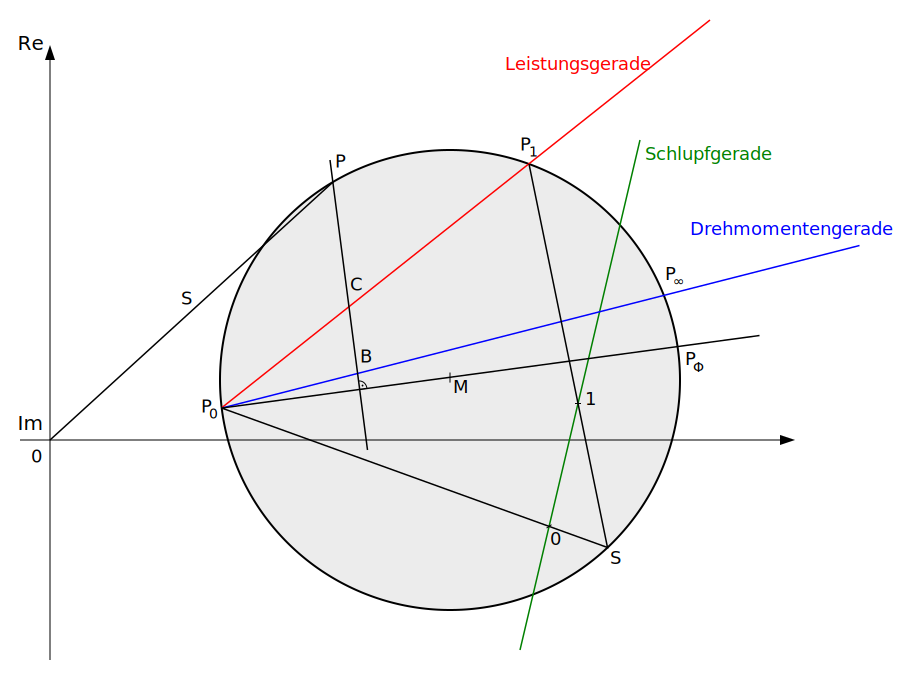
\includegraphics[scale=0.4]{./3_Stand_der_Technik/Abbildungen/Kreisdiagramm_1}
			\caption{Kreisdiagram einer Asynchronmaschine\cite{Wikipedia2024}}
	\end{figure}
	
	
	
	\subsection{Gleichstrommaschine}
	Die Gleichstrommascheine besteht im Stator entweder aus Permanetmagneten, oder aus permanent-erregten Erregerwicklung. Der Rotor besteht aus Wicklungen, welche durch einen Kommutator (auch Stromwender genannt) und B�rsten mithilfe von Gleichspannung versorgt werden. Die Drehzahl der Maschine kann hierbei ganz einfach durch Ver�ndern der Versorgungsspannung linear geregelt werden. 
	
	\begin{figure}[H]
			\centering
			\includegraphics[scale=0.8]{./3_Stand_der_Technik/Abbildungen/Gleichstrommaschine_1}
			\caption{Aufbau Gleichstrommaschine\cite{Pischtschan2024}}
	\end{figure}
	
	Vorteil des Gleichstrommotors ist seine einfach Drehzahlregelung durch Ver�nderung der Spannung, Nachteil der hohe Wartungsaufwand und Verschlei� der Maschine. Er wird aufgrund von sinkenden Preisen bei Frequenzumrichtern immer weniger verwendet.
	
	\subsection{Synchronmaschine}
	Die Synchronmaschien ist �hnlich wie die Asynchronmaschine aufgebaut, sie l�uft jedoch immer synchron mit ihrem Drehfeld. Zur Regelung der Synchronmaschine ist ein Frequenzumrichter unbedingt n�tig. Aufgrund der sinkenden Kosten von Frequenzumrichtern, wird die Synchronmaschine immer weiter verbreitet. Mithilfe eines guten Frequenzumrichters ist es m�glich Drehmoment oder Drehzahl genau zu regeln. Synchronmaschinen erzeugen beim Betrieb eine elektromagnetische Kraft, welche wie ein Geneartor wirkt. Diese Kraft kann gemessen werden und nennt sich Back-EMF.\cite{zikodrive.com2024} Sie wird im sensorlosen Betrieb von Synchronmaschinen verwendet um die genaue Drehzahl der Maschien zu ermitteln. Die Synchronmaschine ist in einigen verschiedenen Bauformen verbreitet:
	
	\subsubsection{B�rstenlose Gleichstrommaschine (BLDC-Maschine)}
		Die BLDC-Maschine wird verwendet, wenn hohes Drehmoment und hohe Drehzahl ben�tigt wird. Der Rotor besteht aus Permanentmagneten. Die Maschine kann mithilfe einer simplen Schaltung besthend aus 6 MOSFETs einfach geregelt werden.(siehe \ref{Trapezfoermige Regelung}) Die BLDC-Maschine gibt ein Trapezf�rmiges Back-EMF zur�ck.\cite{Rode2023}
		
	\begin{figure}[H]
			\centering
			\includegraphics[scale=0.7]{./3_Stand_der_Technik/Abbildungen/BLDC_Back-EMF_1}
			\caption{Back-EMF BLDC-Maschine\cite{Rode2023}}
	\end{figure}
		
	\subsubsection{Permanent erregte Synchronmaschine (PMSM-Maschine)}
		Die PMSM-Maschine isst vom Aufbau fast gleich wie die BLDC-Maschine, nur sind die Magneten im Rotor anders angeordnet. Diese Maschine kann nur mit FOC-Regelung(siehe \ref{Feldorientierte Regelung}) angesteuert werden, welche in der Regel etwas teuer und aufw�ndiger ist. Sie wird mithilfe von einem sinusf�rmigen Drehfeld geregelt und gibt auch ein sinusf�rmiges Back-EMF zur�ck. Sie ist effizienter als die BLDC Maschine und kann auch bei sehr niedrigen und sehr hohen Drehzahlen ohne Probleme verwendet werden. Sie wird verwendet wenn es n�tig ist Drehzahl oder Drehmoment genau zu kontrollieren.\cite{Rode2023}
		
	\begin{figure}[H]
			\centering
			\includegraphics[scale=0.5]{./3_Stand_der_Technik/Abbildungen/PMSM_Back-EMF_1}
			\caption{Back-EMF PMSM-Maschine\cite{Rode2023}}
	\end{figure}
		
	\subsubsection{Fremderregte Synchronmaschine (FSM-Maschine)}
		Die fremderregte Synchronmaschine hat nun im Rotor statt Permanentmagneten Erregerwicklungen, welche entweder durch Schleifringe oder �ber einen Luftspalt induziert Energie �bertragen bekommen. Sie werden gro�teils im Generatorbetrieb eingesetzt, da die erzeugte Leistung einfach geregelt werden kann und sie �ber ihren gesamten Leistungsbereich sehr effizient sind.
	
	\subsubsection{Reluktanzmaschine}
		Bei der Reluktanzmaschine besteht der Rotor der Maschine aus Elektroblech. Es wird nicht wie bei �blichen Maschinen das Prinzip der Lorentzkraft sondern ausschlie�lich das der Reluktanzkraft angewandt. Aufgrund dessen hat dieser Motor eine eher geringe Leistungsdichte, ist aber im Gegenzug sehr g�nstig zu fertigen und zu k�hlen.\cite{oswos.com2024}
	
	
	\subsection{Positionsmessung}
	Um Motoren genau Regeln zu k�nnen ist es meistens n�tig die Position des Rototrs zu messen. Dies kann wie folgt umgesetzt werden:

	\subsubsection{Back-EMF}
		Wenn in einer Spule sich der Stromfluss �ndert, wird eine Spannung induziert, im Fall von Synchronmaschinen wird diese Spannung Back-EMF genannt. Diese kann gemessen werden und es kann anhand dieser die Position und Drehzahl des Rotors ermittelt werden.
		
	\begin{figure}[H]
			\centering
			\includegraphics[scale=0.5]{./3_Stand_der_Technik/Abbildungen/PMSM_Back-EMF_1}
			\caption{Back-EMF Synchronmaschine\cite{Rode2023}}
	\end{figure}
	
	\subsubsection{Hall-Sensoren}
		Der Hall-Sensor ist ein magnetotastischer Sensor, er misst das magnetische Gleichfeld innerhalb eines Halbleiterpl�ttchens. Das Feld des Magneten durchsetzt das Pl�ttchen senkrecht, sodass die Ladungstr�ger aus ihrer Bahn abgelenkt werden. Es kann nun eine zum Feld proportionale Hall-Spannung abgegriffen werden.
		
		\begin{equation}
			U_{H} =  R_{H}*I*\frac{B}{d}
		\end{equation}
		
		$U_{H} \cdots$ Hallspannung \newline
		$R_{H} \cdots$ Hallkonstante \newline
		$I \cdots$ Pl�ttchenstrom \newline
		$B \cdots$ Induktion \newline
		$d \cdots$ Dicke des Pl�ttchens \newline
		
		Indem man 3 solcher Hall Sensoren hinter einem Motor anbringt kann so die Position und Drehzahl des Motors gemessen werden. Die Genauigkeit der Positionsmesung h�ngt dabei von der Anzahl der Polpaare ab. Desto mehr, desto genauer ist die Messung\cite{JulinHorstkoetter2023}
		
		\begin{figure}[H]
			\centering
			\includegraphics[scale=0.5]{./3_Stand_der_Technik/Abbildungen/Hall-Sensor_1}
			\caption{Ausgangssignal der Hallsensoren je nach Winkel des Rotors\cite{JulinHorstkoetter2023}}
		\end{figure}
	
	\subsubsection{Resolver / Drehgeber}
		Resolver oder Drehgeber sind beide Sensoren zur genauen Ermittlung der Motorposition. Die Genauigkeit h�ngt nur noch von der Bauweise des Sonsors ab und nicht von der des Motors. Sie k�nnen beide Inkremental oder Absolut den Winkel des Motors angeben. Der Unterschied zwischen beiden liegt darin, dass der Drehgeber ein digitales Signal ausgibt und der Resolver ein analoges.
	
	\subsection{Trapezf�rmige Regelung}\label{Trapezfoermige Regelung}
%%BLDC Motor wird auch Blockstrommotor genannt
%%evtl noch Schrittmotor inkludieren
	
	\subsection{Feldorientierte Regelung (FOC)}\label{Feldorientierte Regelung}
	Mithilfe der feldorientiereten Regelung ist es m�glich das Feld des Stators so anzupassen, dass es dem Feld des Rotors genau so vorl�uft, dass Drehmoment und Effizienz maximiert werden. Im Gegensatz zur BLDC-Regelung kann das Statorfeld nicht nur 6 Positionen annehmen, sondern unbegrenzt viele. Man kann mit dieser Methode auch eine etwas h�here Drehzahl erreichen. Um diese 90� Verschiebung des Statorfelds zu erreichen, wird der Feldvektor zun�chst in seine zwei Komponenten Id und Iq aufgeteilt:
	
	\begin{figure}[H]
			\centering
			\includegraphics[scale=0.3]{./3_Stand_der_Technik/Abbildungen/FOC_Control_1}
			\caption{Komponenten des Statormagnetfelds\cite{MATLAB2020}}
	\end{figure}
	
	Das Ziel des Reglers ist demnach Id gegen 0 zu regeln und Iq entsprechend dem gew�nschten Drehmoment so hoch wie m�glich zu regeln.
	
	Der Aufbau eines FOC-Algorhitmus ist in der Regel wiefolgt:
	
	\begin{figure}[H]
			\centering
			\includegraphics[scale=0.3]{./3_Stand_der_Technik/Abbildungen/FOC_Control_2}
			\caption{Aufbau eines FOC-Algorhitmus\cite{MATLAB2021}}
	\end{figure}
	
	Mithilfe von Shunts wird der derzeitige Strom zum Motor gemessen. Diese Werte werden mithilfe von mathematischen Transformationen (Clark- und Park Transformation) in die zwei Anteile Id und Iq aufgeteilt. Auch wird mithilfe eines Positionssensors die Position des Rotors gemessen.
	Zwei PI-Regler regeln nun Id auf 0 und Iq auf den gew�nschten Strom. Anschlie�end werden die Werte mithilfe von mathematischen Transformationen(inverse Clark Transformation) in die gew�nschten Spannungswerte Vd und Vq umgerechnet. 